{
    \subsection{Արդյունքներ}\label{subsec:results}
    Ստորև ներկայացված է առաջատար այլ գործիքների և
    նոր մշակված գործիքի արդյունավետության աղյուսակը (Աղյուսակ \ref{tab:juliet_test}):
    \begin{table}[h!]
    \centering
    \begin{tabularx}{\textwidth}{|*{6}{>{\centering\arraybackslash}X|}}
        \hline
        \textbf{Name} & \textbf{True Positives} & \textbf{True Negatives} & \textbf{False Positives} & \textbf{False Negatives} & \textbf{F1 score} \\
        \hline
        \textbf{CSA} & 536 & 4481 & 125 & 332 & 0.7011 \\
        \hline
        \textbf{Infer} & 262 & 4392 & 214 & 606 & 0.3899 \\
        \hline
        \textbf{SMOKE} & 496 & 4510 & 96 & 372 & 0.6795 \\
        \hline
        \textbf{PCA} & 486 & 4342 & 264 & 382 & 0.6007 \\
        \hline
        \textbf{SVF} & 452 & 4168 & 438 & 416 & 0.5142 \\
        \hline
        \rowcolor{yellow!100} \textbf{MLH} & 868 & 4606 & 0 & 0 & 1 \\
        \hline
    \end{tabularx}
    \caption{Juliet թեստերի հավաքածույի վրա համեմատման արդյունքների}
    \label{tab:juliet_test}
\end{table}

    \subsubsection{Դինամիկ հիշողության արտահոսքի հայտնաբերումը առաջատար բաց կոդով գործիքներում}
    Մի շարք հատուկ առանձնացված բաց կոդով գործիքներ դասակարգված են ըստ իրենց ակտիվության և կարևորության։ Այդ գործիքներից
    ավելի քան հարյուրը թեստավորվել են նոր մշակված գործիքի միջոցով՝ դինամիկ հիշողության արտահոսքի խնդիրները հայտնաբերելու
    նպատակով։ Ստացված ճիշտ արդյունքները հրապարակվել և
    հաստատվել են, սխալ ստացված արդյունքների համար կատարվել է վերլուծություն և մշակվել հետագա պլան գործիքում առկա
    թերությունները վերացնելու նպատակով։ Նկար \ref{fig:figure4}-ում ներկայացված է ֆունկցիայի օրինակ
    coturn\cite{COTURN}-ից, որում հարցումների համակարգի API-ի օգտագործմամբ գրված
    սստուգիչի կողմից հայտնաբերվել է դինամիկ հիշողության արտահոսքի դեպք։

    \begin{figure}[h]
        \centering
        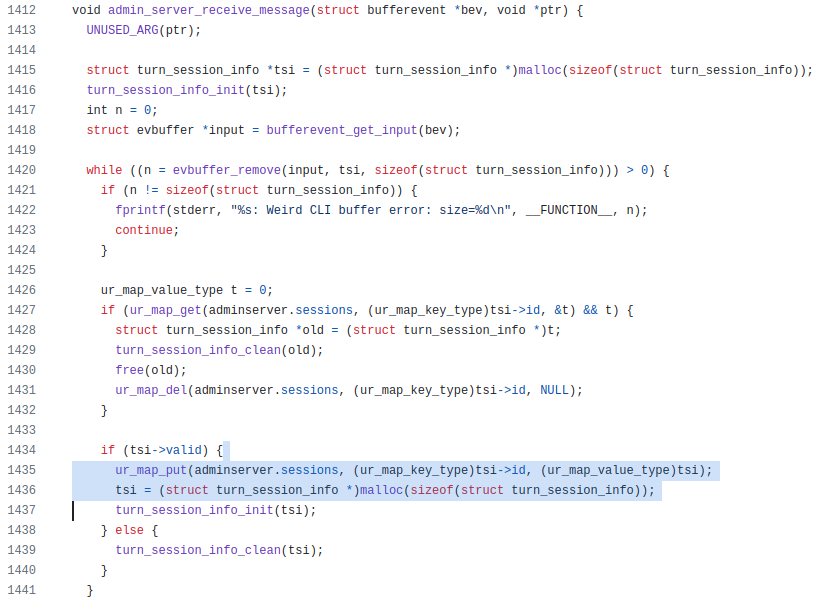
\includegraphics[width=1\textwidth]{pic4}
        \caption{Դինամիկ հիշողության արտահոսքի իրական օրինակ}
        \label{fig:figure4}
    \end{figure}
}